% Actualization Chain Diagram — Static LaTeX figure for the dissertation
% Simplified, clean mirror of the v10 interactive HTML (gold-synced §§1-4).
% Three-column vertical layout: kinetic roles (left) | chain (center) | time (right),
% all within the all-encompassing Motion-and-Time horizon.
%   - A3 split: cognitive actuality + an orthogonal Doxa bubble beneath it.
%   - Doxa -> Emotion (emotion is the doxastic ratification of evaluatively
%     complex content); Emotion -> A2 (judgment-modifying feedback).
%   - Hexeis -> M2->A3 (dispositions condition the cognitive motion) and
%     A4 -> Hexeis (action sediments disposition).
%   - Gold-sync: aisthēsis-as-kinēsis (direct, not analogical); naming
%     principle = Phys. V.5, 229a24-25; A1 = resonant aisthēma + resonant epithymia;
%     M1->A2 = resonant kinēsis crystallizes into the phantasma.
% Compile with: pdflatex (requires tikz, amsmath)

\documentclass[border=24pt,tikz]{standalone}
\usepackage[T1]{fontenc}
\usepackage{amsmath}
\usepackage{tikz}
\usetikzlibrary{
  arrows.meta,
  positioning,
  calc,
  decorations.pathreplacing,
  fit,
  backgrounds,
  shapes.geometric
}

\definecolor{actuality}{RGB}{30,60,120}
\definecolor{motion}{RGB}{140,40,40}
\definecolor{timecolor}{RGB}{60,120,60}
\definecolor{pathoscolor}{RGB}{160,120,40}
\definecolor{emotioncolor}{RGB}{140,60,100}
\definecolor{perceptual}{RGB}{225,237,252}
\definecolor{cognitive}{RGB}{252,240,225}
\definecolor{loopcolor}{RGB}{100,100,100}

\begin{document}
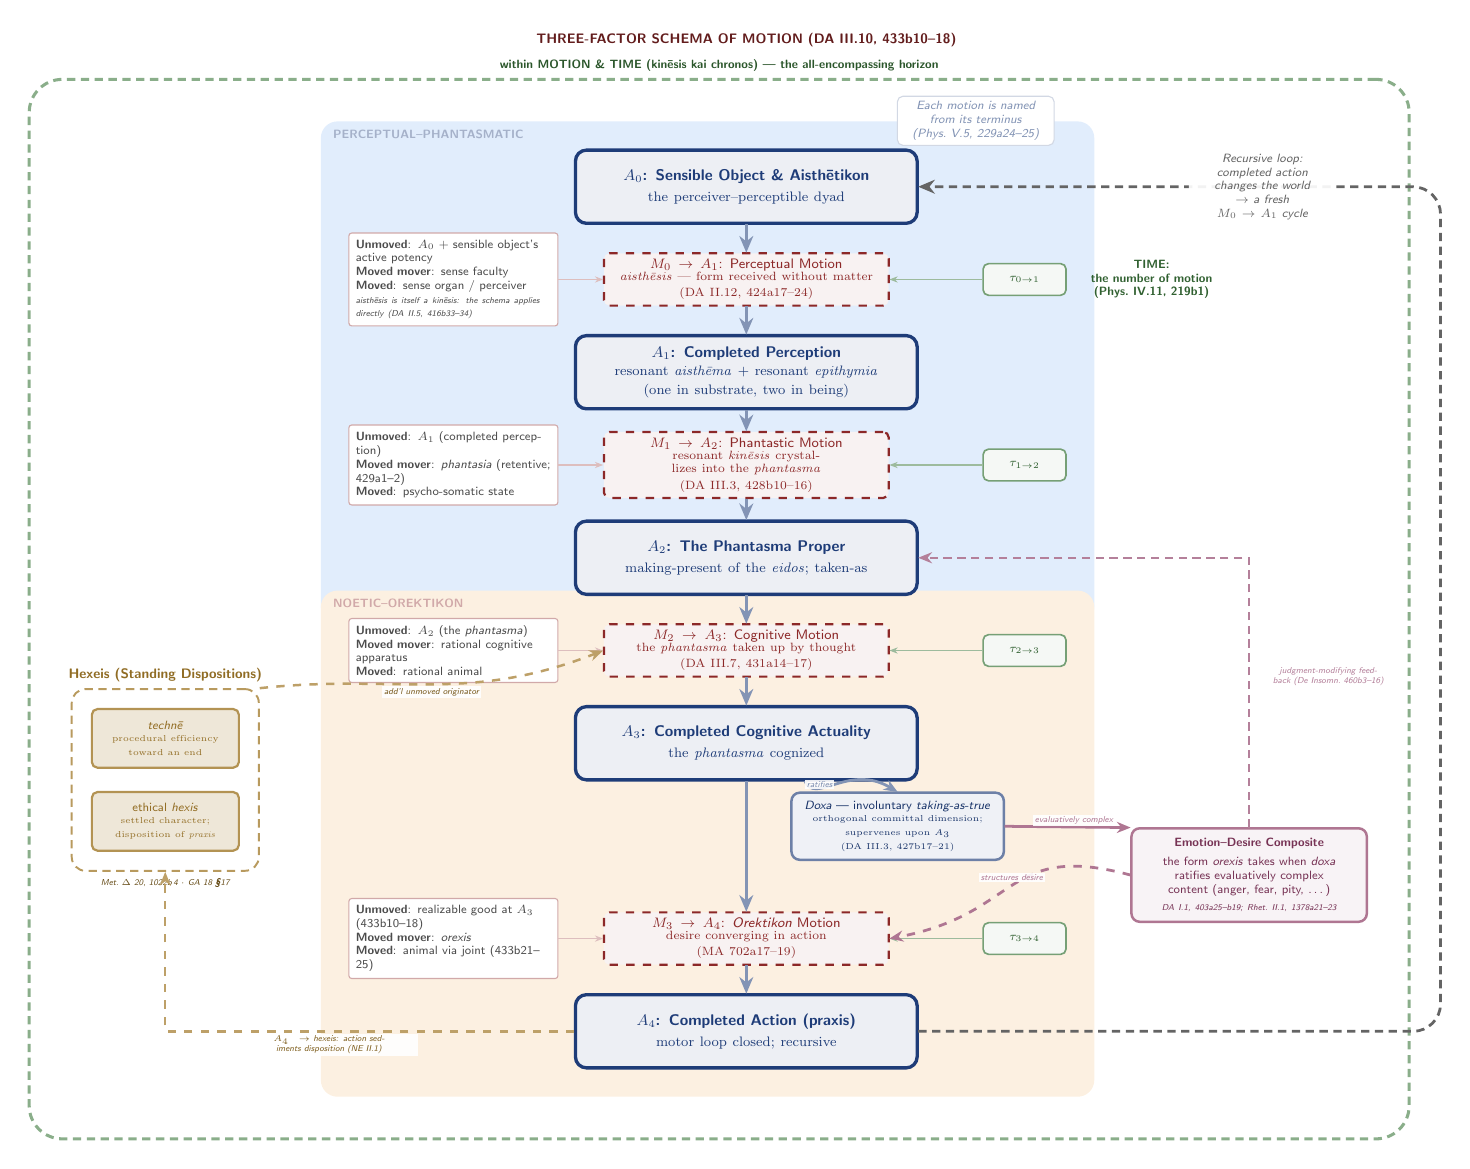
\begin{tikzpicture}[scale=0.62, transform shape,
  actnode/.style={
    rectangle, rounded corners=4pt,
    draw=actuality, fill=actuality!8,
    line width=1.2pt,
    minimum width=7cm, minimum height=1.5cm,
    text width=6.6cm, align=center,
    font=\sffamily\small\bfseries,
    text=actuality
  },
  motionnode/.style={
    rectangle, rounded corners=2pt,
    draw=motion, fill=motion!6,
    line width=0.8pt, dashed,
    minimum width=5.8cm, minimum height=1cm,
    text width=5.6cm, align=center,
    font=\sffamily\footnotesize,
    text=motion
  },
  doxabox/.style={
    rectangle, rounded corners=3pt,
    draw=actuality!65, fill=actuality!7,
    line width=0.9pt,
    minimum width=4.2cm,
    text width=4.0cm, align=center,
    font=\sffamily\scriptsize,
    text=actuality!88!black, inner sep=5pt
  },
  timenode/.style={
    rectangle, rounded corners=2pt,
    draw=timecolor!70, fill=timecolor!5,
    line width=0.6pt,
    minimum width=1.7cm, minimum height=0.65cm,
    align=center,
    font=\sffamily\scriptsize\itshape,
    text=timecolor!80!black
  },
  kineticbox/.style={
    rectangle, rounded corners=1pt,
    draw=motion!40, fill=white,
    line width=0.4pt,
    text width=4.0cm, align=left,
    font=\sffamily\scriptsize,
    text=black!70, inner sep=4pt
  },
  emotionbox/.style={
    rectangle, rounded corners=3pt,
    draw=emotioncolor!70, fill=emotioncolor!6,
    line width=0.9pt,
    text width=4.4cm, align=center,
    font=\sffamily\scriptsize,
    text=emotioncolor!85!black, inner sep=6pt
  },
  hexsub/.style={
    rectangle, rounded corners=2pt,
    draw=pathoscolor!80, fill=pathoscolor!18,
    line width=0.8pt,
    minimum width=3.0cm, minimum height=1.2cm,
    text width=2.8cm, align=center,
    font=\sffamily\scriptsize, text=pathoscolor!92!black, inner sep=3pt
  },
  chainlink/.style={
    -{Stealth[length=6pt,width=5pt]},
    line width=1.3pt, color=actuality!55
  },
  committalarrow/.style={
    -{Stealth[length=5pt,width=4pt]},
    line width=1.0pt, color=actuality!55
  },
  doxaemotion/.style={
    -{Stealth[length=5pt,width=4pt]},
    line width=1.0pt, color=emotioncolor!70
  },
  feedbackarrow/.style={
    -{Stealth[length=5pt,width=4pt]},
    line width=0.9pt, color=emotioncolor!65, densely dashed
  },
  hexisarrow/.style={
    -{Stealth[length=5pt,width=4pt]},
    line width=0.9pt, color=pathoscolor!70, dashed
  },
  looparrow/.style={
    -{Stealth[length=6pt,width=5pt]},
    line width=1pt, color=loopcolor, densely dashed
  },
  tinylabel/.style={
    font=\sffamily\tiny\itshape, inner sep=1pt,
    fill=white, fill opacity=0.9, text opacity=1
  },
]

% ---- Layout constants ----
\def\nodesep{3.8}        % vertical gap between actuality nodes
\def\motionoff{1.9}      % offset of motion nodes from the actuality above
\def\kinoff{6.0}         % kinetic boxes: distance LEFT of center
\def\timeoff{5.7}        % time boxes: distance RIGHT of center
\def\doxagap{2.1}        % extra room opened below A3 for the Doxa bubble

% Schema label — top, centered (above the horizon frame)
\node[motion!70!black, font=\sffamily\footnotesize\bfseries]
  at (0, 3.0)
  {THREE-FACTOR SCHEMA OF MOTION (DA III.10, 433b10--18)};

% ============================================================
%  ACTUALITIES (center column) — mirrors the HTML A0..A4
% ============================================================

\node[actnode] (A0) at (0, 0) {
  $A_0$: Sensible Object \& \textit{Aisth\=etikon}\\[1pt]
  {\footnotesize\normalfont the perceiver--perceptible dyad}
};
\node[actnode] (A1) at (0, -\nodesep) {
  $A_1$: Completed Perception\\[1pt]
  {\footnotesize\normalfont resonant \textit{aisth\=ema} + resonant \textit{epithymia}\\
   (one in substrate, two in being)}
};
\node[actnode] (A2) at (0, -2*\nodesep) {
  $A_2$: The \textit{Phantasma} Proper\\[1pt]
  {\footnotesize\normalfont making-present of the \textit{eidos}; taken-as}
};
\node[actnode] (A3) at (0, -3*\nodesep) {
  $A_3$: Completed Cognitive Actuality\\[1pt]
  {\footnotesize\normalfont the \textit{phantasma} cognized}
};
\node[actnode] (A4) at (0, -4*\nodesep - \doxagap) {
  $A_4$: Completed Action (\textit{praxis})\\[1pt]
  {\footnotesize\normalfont motor loop closed; recursive}
};

% ============================================================
%  MOTIONS (between actualities)
% ============================================================

\node[motionnode] (M01) at (0, -\motionoff) {
  $M_0 \!\to\! A_1$: Perceptual Motion\\[-1pt]
  {\scriptsize\normalfont\textit{aisth\=esis} --- form received without matter\\(DA II.12, 424a17--24)}
};
\node[motionnode] (M12) at (0, -\nodesep - \motionoff) {
  $M_1 \!\to\! A_2$: Phantastic Motion\\[-1pt]
  {\scriptsize\normalfont resonant \textit{kin\=esis} crystallizes into the \textit{phantasma}\\(DA III.3, 428b10--16)}
};
\node[motionnode] (M23) at (0, -2*\nodesep - \motionoff) {
  $M_2 \!\to\! A_3$: Cognitive Motion\\[-1pt]
  {\scriptsize\normalfont the \textit{phantasma} taken up by thought\\(DA III.7, 431a14--17)}
};
\node[motionnode] (M34) at (0, -3*\nodesep - \motionoff - \doxagap) {
  $M_3 \!\to\! A_4$: \textit{Orektikon} Motion\\[-1pt]
  {\scriptsize\normalfont desire converging in action\\(MA 702a17--19)}
};

% ============================================================
%  CHAIN ARROWS
% ============================================================

\draw[chainlink] (A0.south) -- (M01.north);
\draw[chainlink] (M01.south) -- (A1.north);
\draw[chainlink] (A1.south) -- (M12.north);
\draw[chainlink] (M12.south) -- (A2.north);
\draw[chainlink] (A2.south) -- (M23.north);
\draw[chainlink] (M23.south) -- (A3.north);
\draw[chainlink] (A3.south) -- (M34.north);
\draw[chainlink] (M34.south) -- (A4.north);

% ============================================================
%  TIME (right column) — interval notation only
% ============================================================

\node[timenode] (T01) at (\timeoff, -\motionoff) {$\tau_{0 \to 1}$};
\node[timenode] (T12) at (\timeoff, -\nodesep - \motionoff) {$\tau_{1 \to 2}$};
\node[timenode] (T23) at (\timeoff, -2*\nodesep - \motionoff) {$\tau_{2 \to 3}$};
\node[timenode] (T34) at (\timeoff, -3*\nodesep - \motionoff - \doxagap) {$\tau_{3 \to 4}$};

\foreach \t/\m in {T01/M01, T12/M12, T23/M23, T34/M34} {
  \draw[-{Stealth[length=3pt]}, timecolor!50, thin] (\t.west) -- (\m.east);
}

\node[timecolor!80!black, font=\sffamily\scriptsize\bfseries,
  text width=2.6cm, align=center]
  at (\timeoff + 2.6, -\motionoff)
  {TIME:\\the number of motion\\(Phys.\ IV.11, 219b1)};

% ============================================================
%  KINETIC ROLES (left column) — the three factors per motion
% ============================================================

\node[kineticbox] (K01) at (-\kinoff, -\motionoff) {
  \textbf{Unmoved}: $A_0$ + sensible object's active potency\\
  \textbf{Moved mover}: sense faculty\\
  \textbf{Moved}: sense organ / perceiver\\
  {\tiny\itshape \textit{aisth\=esis} is itself a \textit{kin\=esis}: the schema applies directly (DA II.5, 416b33--34)}
};
\node[kineticbox] (K12) at (-\kinoff, -\nodesep - \motionoff) {
  \textbf{Unmoved}: $A_1$ (completed perception)\\
  \textbf{Moved mover}: \textit{phantasia} (retentive; 429a1--2)\\
  \textbf{Moved}: psycho-somatic state
};
\node[kineticbox] (K23) at (-\kinoff, -2*\nodesep - \motionoff) {
  \textbf{Unmoved}: $A_2$ (the \textit{phantasma})\\
  \textbf{Moved mover}: rational cognitive apparatus\\
  \textbf{Moved}: rational animal
};
\node[kineticbox] (K34) at (-\kinoff, -3*\nodesep - \motionoff - \doxagap) {
  \textbf{Unmoved}: realizable good at $A_3$ (433b10--18)\\
  \textbf{Moved mover}: \textit{orexis}\\
  \textbf{Moved}: animal via joint (433b21--25)
};

\foreach \k/\m in {K01/M01, K12/M12, K23/M23, K34/M34} {
  \draw[-{Stealth[length=3pt]}, motion!30, thin] (\k.east) -- (\m.west);
}

% ============================================================
%  DOXA — orthogonal committal dimension, beneath A3
% ============================================================

\node[doxabox] (DOXA) at (3.1, -3*\nodesep - 1.7) {
  \textit{Doxa} --- involuntary \textit{taking-as-true}\\[1pt]
  {\tiny\normalfont orthogonal committal dimension;\\
   supervenes upon $A_3$ (DA III.3, 427b17--21)}
};

% A3 -> Doxa : the cognitive content is (optionally) ratified as true
\draw[committalarrow]
  ($(A3.south) + (1.2, 0)$) .. controls +(0.2, -0.5) and +(-1.0, 0.6) .. (DOXA.north)
  node[pos=0.5, left=1pt, tinylabel, text=actuality!60] {ratifies};

% ============================================================
%  EMOTION-DESIRE COMPOSITE (right) — fed directly by Doxa
% ============================================================

\node[emotionbox] (emotion) at (\timeoff + 4.6, -3*\nodesep - 2.7) {
  \textbf{Emotion--Desire Composite}\\[3pt]
  {\scriptsize the form \textit{orexis} takes when \textit{doxa} ratifies
   evaluatively complex content (anger, fear, pity, \ldots)}\\[2pt]
  {\tiny\itshape DA I.1, 403a25--b19; \textit{Rhet.}\ II.1, 1378a21--23}
};

% Doxa -> Emotion : emotion is fed directly by doxastic ratification
\draw[doxaemotion]
  (DOXA.east) -- (emotion.north west)
  node[pos=0.55, above=0pt, tinylabel, text=emotioncolor!70] {evaluatively complex};

% Emotion -> M34 : emotion structures desire into the orektikon motion
\draw[doxaemotion, dashed]
  (emotion.west) .. controls +(-2.6, 0.7) and +(2.7, 0.5) .. (M34.east)
  node[pos=0.5, above=1pt, tinylabel, text=emotioncolor!70] {structures desire};

% Emotion -> A2 : judgment-modifying feedback (emotion alters the phantasma)
\draw[feedbackarrow]
  (emotion.north) |- (A2.east)
  node[pos=0.28, right=2pt, tinylabel, text=emotioncolor!65,
       text width=3.0cm, align=center]
       {judgment-modifying feedback (\textit{De Insomn.}\ 460b3--16)};

% ============================================================
%  HEXEIS (Standing Dispositions) — far left, near A3/A4
%  Clean bisected bubble: technē + ethical hexis
% ============================================================

\node[hexsub] (techne-hexis) at (-\kinoff - 5.9, -3*\nodesep + 0.1) {
  \textit{techn\=e}\\[1pt]
  {\tiny\normalfont procedural efficiency\\toward an end}
};
\node[hexsub] (ethical-hexis) at (-\kinoff - 5.9, -3*\nodesep - 1.6) {
  ethical \textit{hexis}\\[1pt]
  {\tiny\normalfont settled character;\\disposition of \textit{praxis}}
};

\node[rectangle, rounded corners=5pt,
      draw=pathoscolor!75, fill=none,
      line width=0.7pt, dash pattern=on 3pt off 2pt,
      fit=(techne-hexis)(ethical-hexis), inner sep=7pt,
      label={[font=\sffamily\footnotesize\bfseries,
              text=pathoscolor!90!black]
             above:\textit{Hexeis} (Standing Dispositions)},
      label={[font=\sffamily\tiny\itshape,
              text=pathoscolor!65!black]
             below:Met.\ $\Delta$ 20, 1022b\,4 $\cdot$ GA 18 \S 17}]
      (hexis-band) {};

% Hexeis -> M2->A3 : dispositions are an additional unmoved originator
% (routed up-right through the clear channel below K23)
\draw[hexisarrow]
  (hexis-band.north east) .. controls +(2.8, 0.3) and +(-2.8, -1.1) .. (M23.west)
  node[pos=0.5, below=1pt, tinylabel, text=pathoscolor!75!black]
       {add'l unmoved originator};

% A4 -> Hexeis : each completed action sediments the standing dispositions
\draw[hexisarrow] (A4.west) -| (hexis-band.south)
  node[pos=0.30, below=1pt, tinylabel, text=pathoscolor!80!black,
       text width=3.6cm, align=center]
       {$A_4 \to$ \textit{hexeis}: action sediments disposition (NE II.1)};

% ============================================================
%  NAMING PRINCIPLE (top right) — gold-synced locus
% ============================================================

\node[rectangle, rounded corners=2pt, draw=actuality!20, fill=white,
  font=\sffamily\scriptsize\itshape, text=actuality!55,
  text width=3.0cm, align=center, inner sep=3pt]
  at (\timeoff - 1.0, 1.35) {
  Each motion is named\\from its terminus\\
  (Phys.\ V.5, 229a24--25)
};

% ============================================================
%  RECURSIVE LOOP (far right): A4 changes the world -> fresh A0
% ============================================================

\draw[looparrow, rounded corners=10pt]
  (A4.east) -- ++(\timeoff + 5.0, 0)
  -- ++(0, 4*\nodesep + \doxagap)
  -- (A0.east)
  node[pos=0.50, right=5pt, font=\sffamily\scriptsize\itshape,
    text=loopcolor, text width=2.8cm, align=center,
    fill=white, fill opacity=0.92, text opacity=1, inner sep=3pt]
  {Recursive loop:\\completed action\\changes the world\\$\to$ a fresh
   $M_0 \!\to\! A_1$ cycle};

% ============================================================
%  BACKGROUND ZONES + ALL-ENCOMPASSING MOTION-AND-TIME HORIZON
% ============================================================

\begin{scope}[on background layer]
  \node[fill=perceptual, rounded corners=6pt, inner sep=10pt,
    fit=(A0)(A2)(K01)(K12)(T01)(T12),
    label={[font=\sffamily\scriptsize\bfseries, text=actuality!40,
      anchor=north west, xshift=4pt, yshift=-2pt]north west:
      PERCEPTUAL--PHANTASMATIC}] (zoneupper) {};

  \node[fill=cognitive, rounded corners=6pt, inner sep=10pt,
    fit=(A3)(A4)(K23)(K34)(T23)(T34)(DOXA),
    label={[font=\sffamily\scriptsize\bfseries, text=motion!40,
      anchor=north west, xshift=4pt, yshift=-2pt]north west:
      NOETIC--OREKTIKON}] (zonelower) {};

  % All-encompassing horizon: motion and time as the horizon of the whole chain
  \node[draw=timecolor!60, line width=1.1pt, densely dashed, rounded corners=12pt,
    inner sep=15pt, fit=(zoneupper)(zonelower)(hexis-band)(emotion),
    label={[font=\sffamily\scriptsize\bfseries\itshape, text=timecolor!72!black]
      above:within MOTION \& TIME (\textit{kin\=esis kai chronos}) --- the all-encompassing horizon}]
    (horizon) {};
\end{scope}

\end{tikzpicture}
\end{document}
